\documentclass[11pt,a4paper]{article}
\usepackage{fontspec}
\setmainfont{TeX Gyre Pagella}
\usepackage[a4paper,margin=2.3cm]{geometry}
\usepackage{graphicx,booktabs,float,caption,array,xcolor,longtable}
\usepackage{xurl}
\usepackage[hidelinks]{hyperref}
\usepackage[round]{natbib}
\usepackage{setspace}
\setstretch{1.05}
\setlength{\parindent}{0pt}
\setlength{\parskip}{0.55em}
\captionsetup{font=small,labelfont=bf}
\hypersetup{pdftitle={Saxton's Atlas, Measured},pdfauthor={Tristan Hotham}}
\begin{document}
\begin{center}
{\Large\bfseries Saxton's Atlas, Measured\par}
\vspace{0.4em}
{\large The accuracy, scale and orientation of the first county atlas of England and Wales (1574 to 1579)\par}
\vspace{1.2em}
{\large Tristan Hotham\par}
\vspace{0.3em}
{\small Independent researcher\\ ORCID: 0000-0003-4931-9349\\ DOI: \url{https://doi.org/10.5281/zenodo.24052723}\par}
\vspace{0.8em}
2026
\end{center}
\begin{quote}\small\textbf{Abstract.} Christopher Saxton's county maps of England and Wales, engraved between 1574 and 1579, are the foundation of English county cartography. I read 857 positions (town and church symbols, castles and bridges) on all 34 county sheets and on the general map in the Biblioth\`eque nationale de France copy, matched them to Wikidata settlement points and fitted each sheet to the ground with similarity, affine and thin-plate spline transformations. At each sheet's own scale and orientation, the median place is misplaced by 1.37 km; 71\% are within 2 km. Sheets differ in quality (median 0.68 to 2.66 km) but hardly at all in shape (median stretch 1.05). True north is turned anticlockwise on 31 of 34 county sheets, by a median of 8.4$^\circ$ (Cornwall excluded), close to the magnetic variation of about 11\textonequarter$^\circ$ east measured in London in 1580, while the general map is turned only -0.9$^\circ$. On the general map the median town is misplaced by 4.2 km, against 17.6 km for the Gough Map of about 1360 measured in the same way.\end{quote}

\section{Introduction}
Saxton's atlas, published in 1579 with a general map of England and Wales and 34 county maps, was the first set of maps of the whole country at county scale drawn from a new survey \citep{evans}. Its sheets were copied, re-engraved and reissued for two centuries. This paper asks three plain questions that a modern reader can test with digital scans and a gazetteer: how close to their true places are the towns; how consistent are the sheets with one another in scale and shape; and which way is north. It follows the method of an earlier study of the Gough Map \citep{gough}, so that the two can be compared.

\section{Data}
The scans are the Wikimedia Commons images of the BnF copy (ark:/12148/btv1b55007148q), 3,840 pixels wide. Of 41 files supplied, 35 are the general map and the 34 county maps, one is a map of Scotland bound with the atlas that is not Saxton's, and 5 are single sheets from other copies duplicating Devon, Dorset, Cornwall, Wiltshire and Somerset; these were identified and set aside. True positions are Wikidata settlement points (CC0), with a handful typed by hand where Wikidata had no settlement item of the right type. Coastlines for figures are from Natural Earth \citep{ne}.

\section{Methods}
\subsection{Reading the sheets}
For each sheet I placed a few anchor towns by eye on an overview, then worked through candidate settlements in the county (cities and market towns first, then towns and villages), each shown as a zoomed crop of the full scan centred on its predicted position (a similarity, then an affine, then a thin-plate spline fit to the towns already read). I accepted a reading only when an engraved symbol and a legible or nearly legible name agreed with the place, and recorded the pixel position of the symbol. Each reading is flagged certain (626), probable (183) or doubtful in its exact point (2). Readings per county sheet range from 7 to 62 (median 22). Every county sheet was read.

\subsection{Fitting}
True positions are projected onto an azimuthal equidistant plane centred on the mean of each sheet's readings, in kilometres, so that up is true north. Pixel positions have $y$ turned upwards. A similarity transformation (one scale, one rotation, a shift) and an affine transformation are fitted by least squares \citep{tobler}. A place's misplacement is the ground distance between its true position and the sheet position taken back through the inverse of the sheet's own similarity; the same for the affine. Readings misplaced by more than the larger of 5 km and four times the sheet median (25 km on the general map) are treated as misreadings and dropped (0 in all). A thin-plate spline \citep{bookstein} with smoothing equal to the number of readings bends a true 5 km grid onto each sheet and gives a leave-one-out check. The turn is the angle of the similarity's rotation: positive when true north points to the left of the sheet's top. Places read on two county sheets give a sheet-to-sheet check.

\section{Results}
\begin{figure}[H]\centering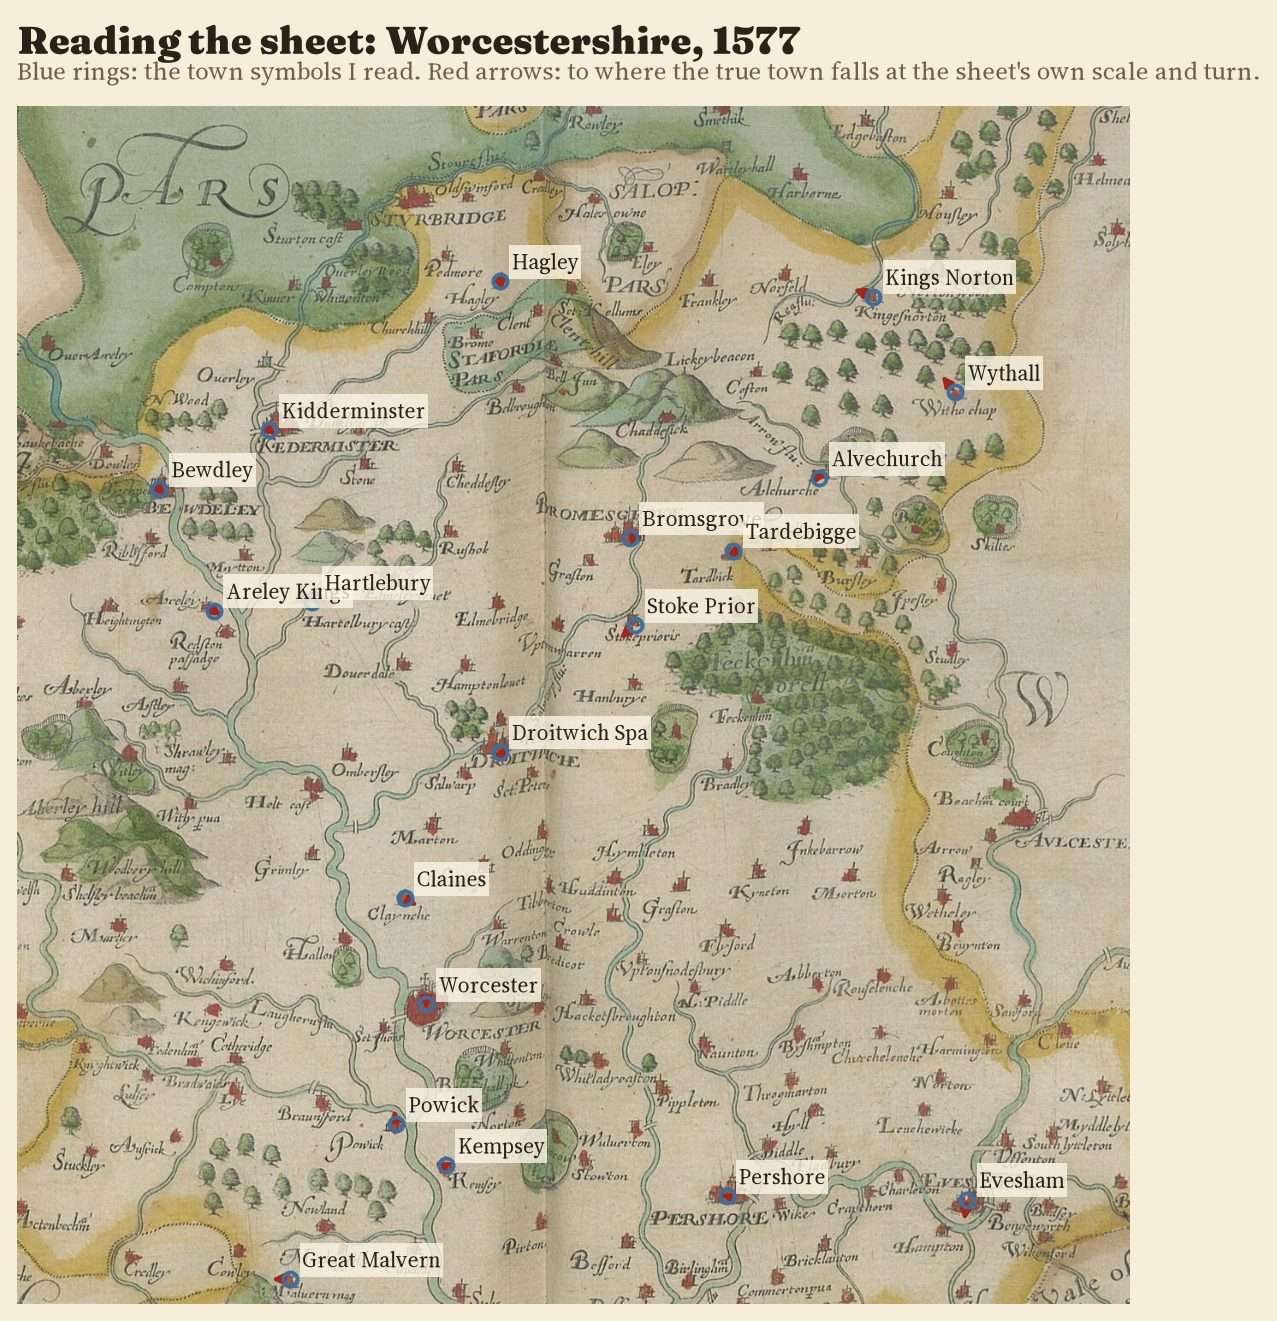
\includegraphics[width=.92\linewidth]{f_reading.jpg}\caption{Readings on the Worcestershire sheet (1577). Arrows run from each reading to where the true town falls under the sheet's similarity fit.}\end{figure}
\subsection{Accuracy}
Across 811 readings on county sheets, the median misplacement is 1.37 km (mean 1.59 km); 32\% are within 1 km and all but 5 within 5 km. The affine fit lowers the median only to 1.28 km, and the thin-plate spline's leave-one-out median is 1.29 km. Certain readings give 1.35 km, probable ones 1.55 km. By region: South-west 1.34 km (135 readings); South-east 1.36 km (77 readings); East 1.72 km (89 readings); Midlands 1.12 km (187 readings); North 1.48 km (160 readings); Wales 1.58 km (163 readings). The largest misplacements are Wisbech on Northants and Cambs (7.8 km), March on Northants and Cambs (7.4 km), Aberystwyth on Mid and south Wales (5.4 km), Newport on Mid and south Wales (5.1 km). Part of every figure is the gap between a modern Wikidata point and the sixteenth century church symbol, typically a few hundred metres.
\begin{figure}[H]\centering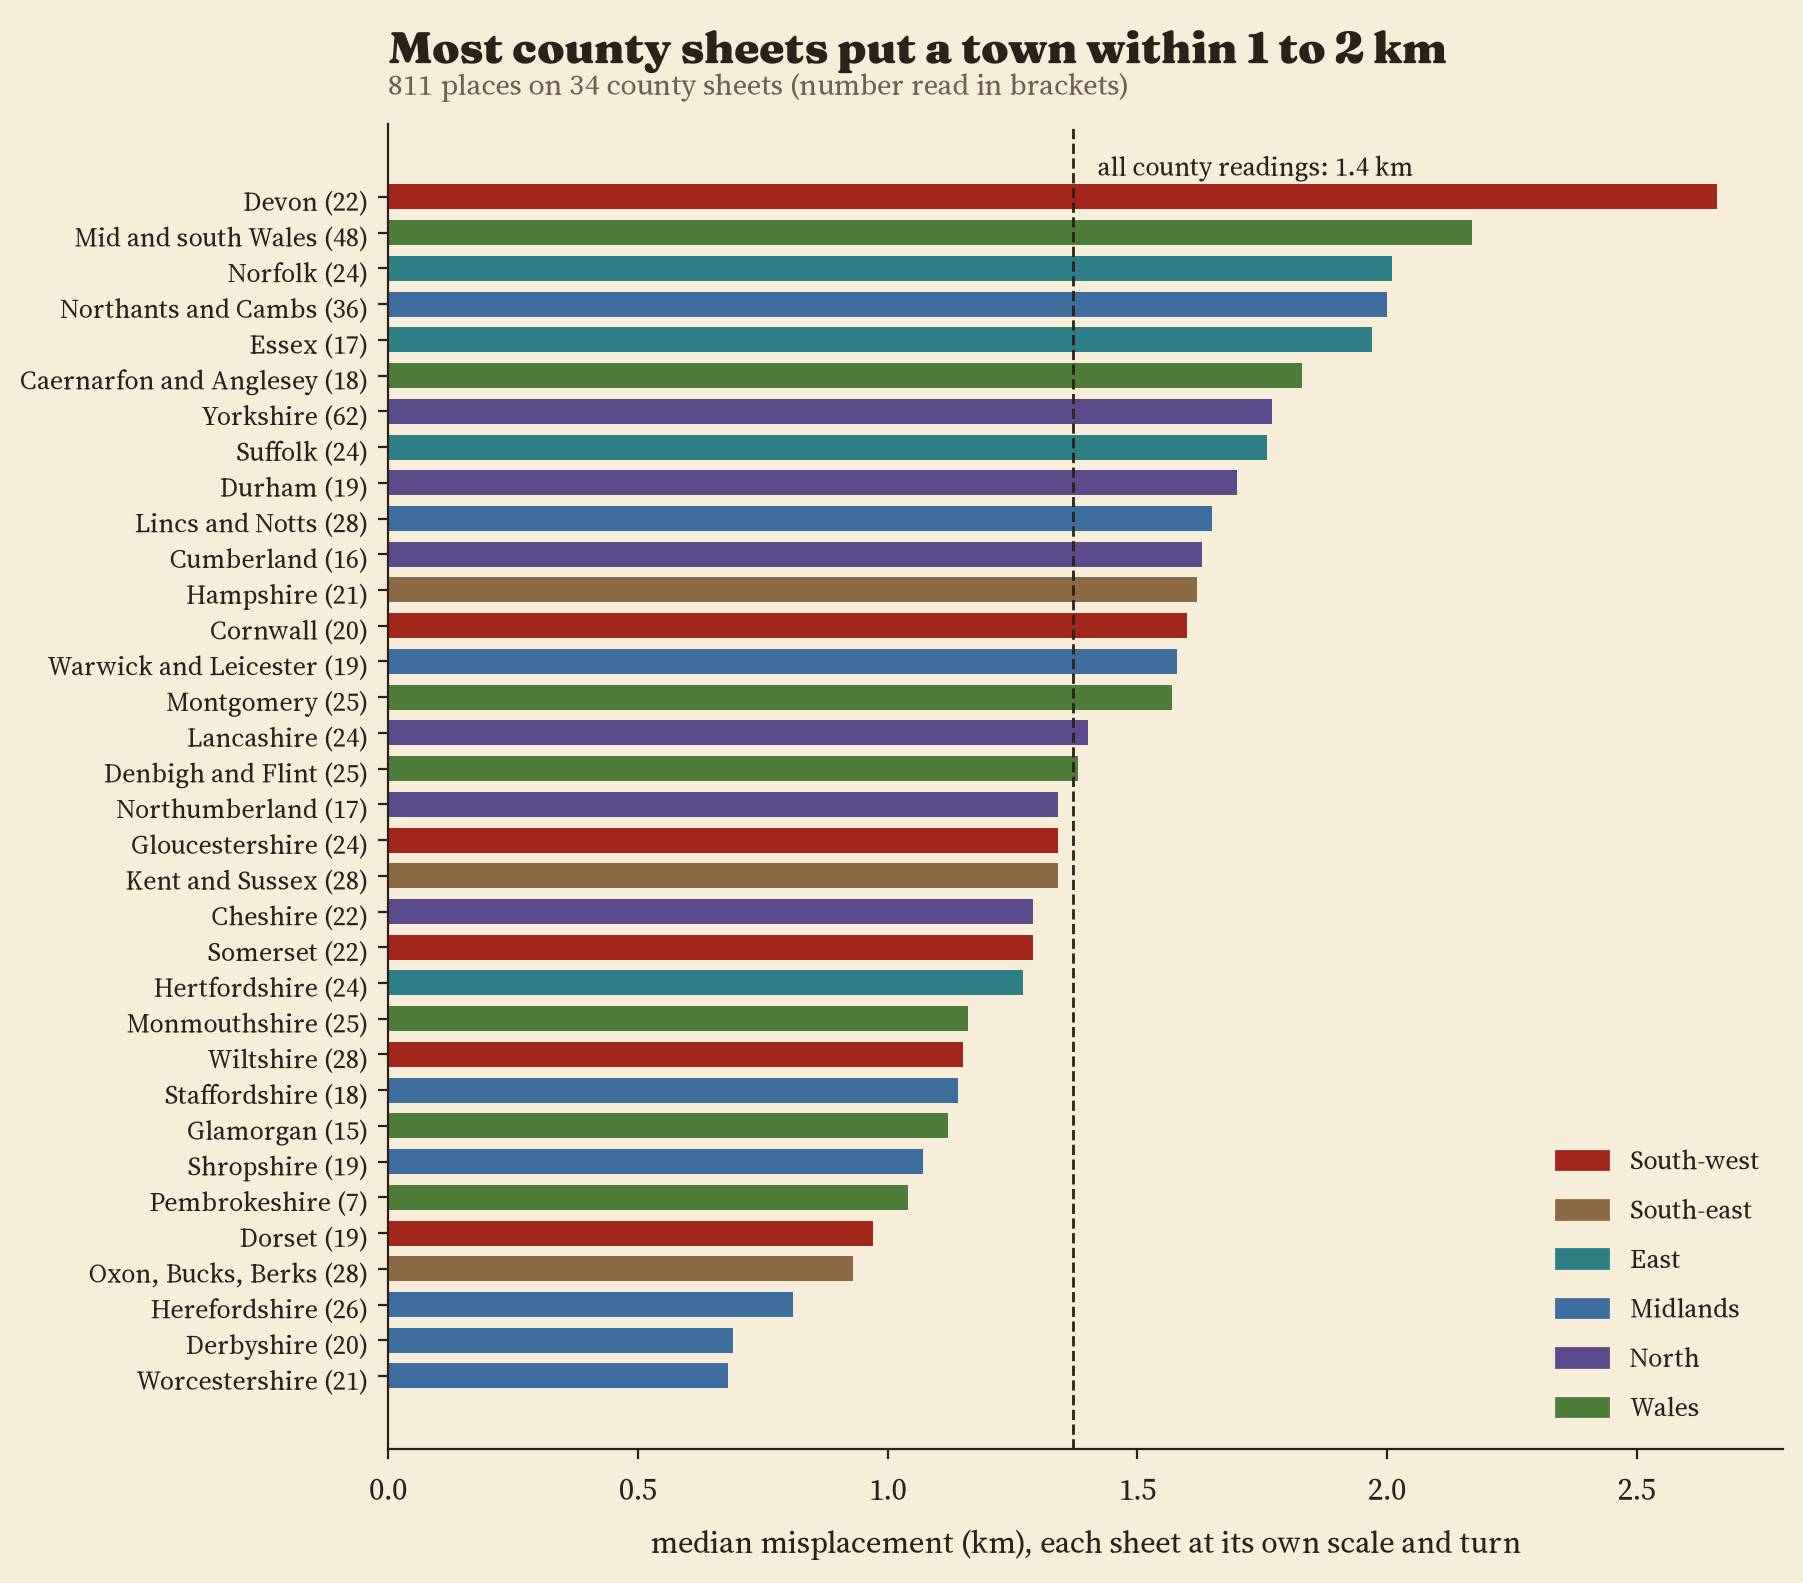
\includegraphics[width=.8\linewidth]{f_errors.png}\caption{Median misplacement per county sheet.}\end{figure}
\begin{figure}[H]\centering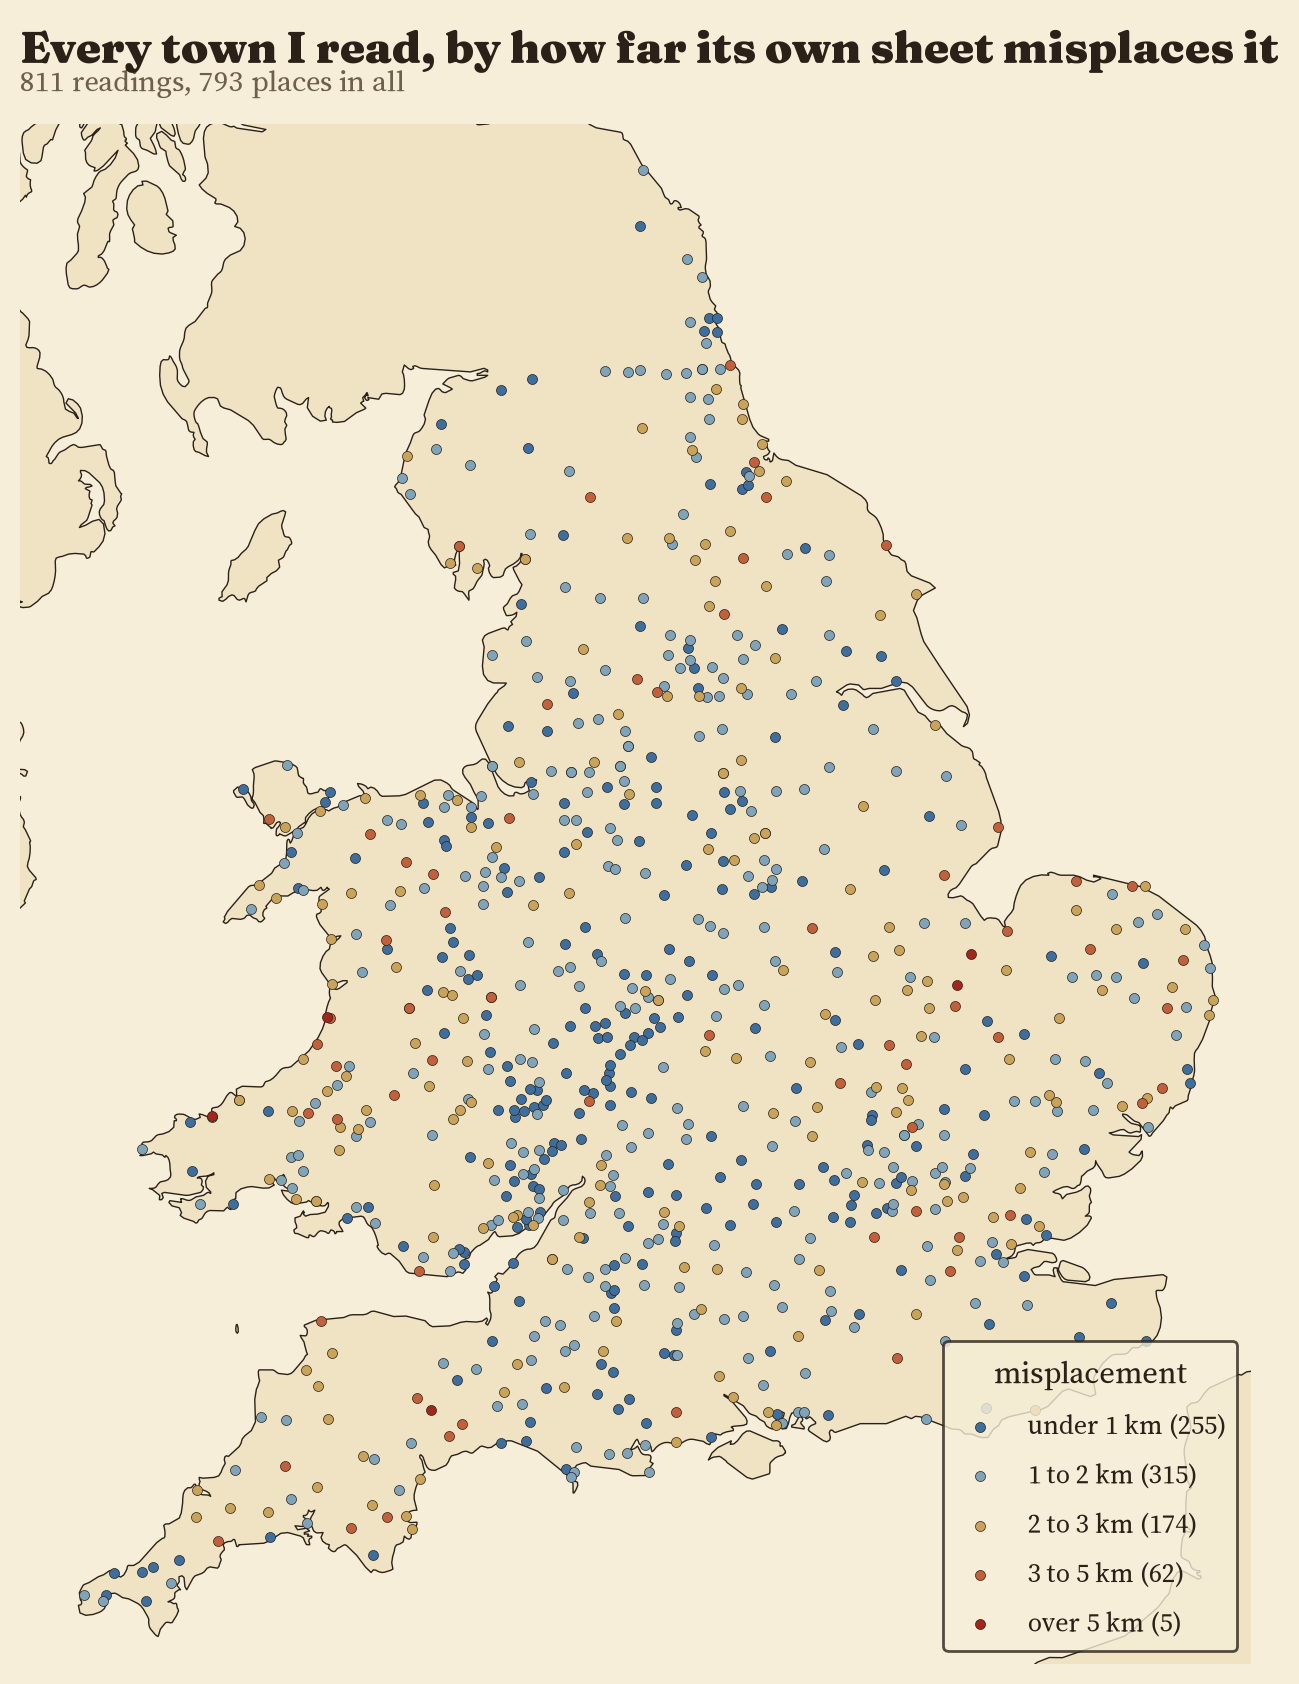
\includegraphics[width=.72\linewidth]{f_map.png}\caption{Every reading on a county sheet, coloured by misplacement.}\end{figure}

\subsection{Scale and shape}
Scales range from 17.6 scan pixels per km (Yorkshire) to 46.1 (Hertfordshire), a factor of 2.6: Saxton fitted each county to the plate rather than keeping one scale. The median affine stretch is 1.05 and the largest 1.16 (Denbigh and Flint). 16 places read on two sheets fall a median 2.30 km apart when each is taken to the ground through its own sheet (largest Llanidloes, 5.2 km).
\begin{figure}[H]\centering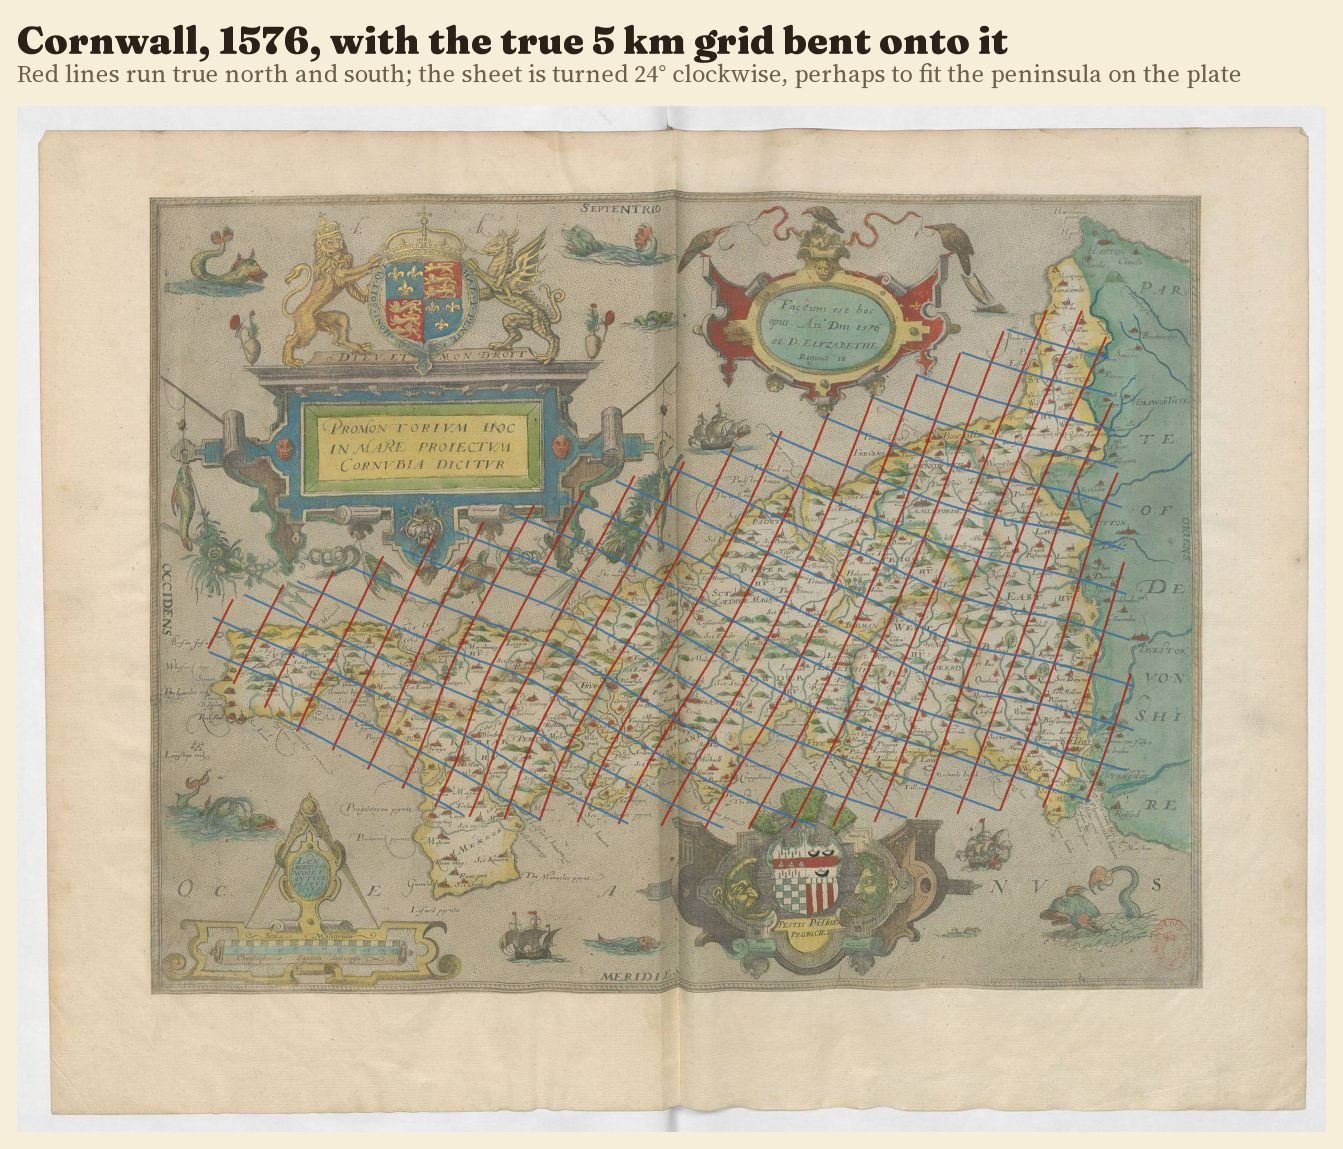
\includegraphics[width=.8\linewidth]{f_grid.jpg}\caption{The Cornwall sheet with the true 5 km grid bent onto it by the thin-plate spline.}\end{figure}

\subsection{Orientation}
True north is turned anticlockwise on 31 of 34 county sheets; leaving aside Cornwall (-24.0$^\circ$; possibly turned so the long peninsula fits the plate), the median is 8.4$^\circ$ and the middle half lies between 7.6$^\circ$ and 10.0$^\circ$; 28 sheets lie between 5$^\circ$ and 16$^\circ$. The exceptions are Devon (-3.1°), Cornwall (-24.0°), Warwick and Leicester (-9.7°). William Borough measured the variation of the compass at Limehouse in October 1580 as about 11\textonequarter$^\circ$ east \citep{borough, eb1911}. If Saxton's surveys were oriented by magnetic compass and the plates drawn with magnetic north at the top, true north would appear turned anticlockwise by about that amount, as observed. The general map, compiled from the county sheets, is turned only -0.9$^\circ$, which suggests it was set to true north when it was put together. The scans themselves may be skewed by a degree or so; this does not change the pattern. The explanation is offered as a reading of the evidence, not a proof.
\begin{figure}[H]\centering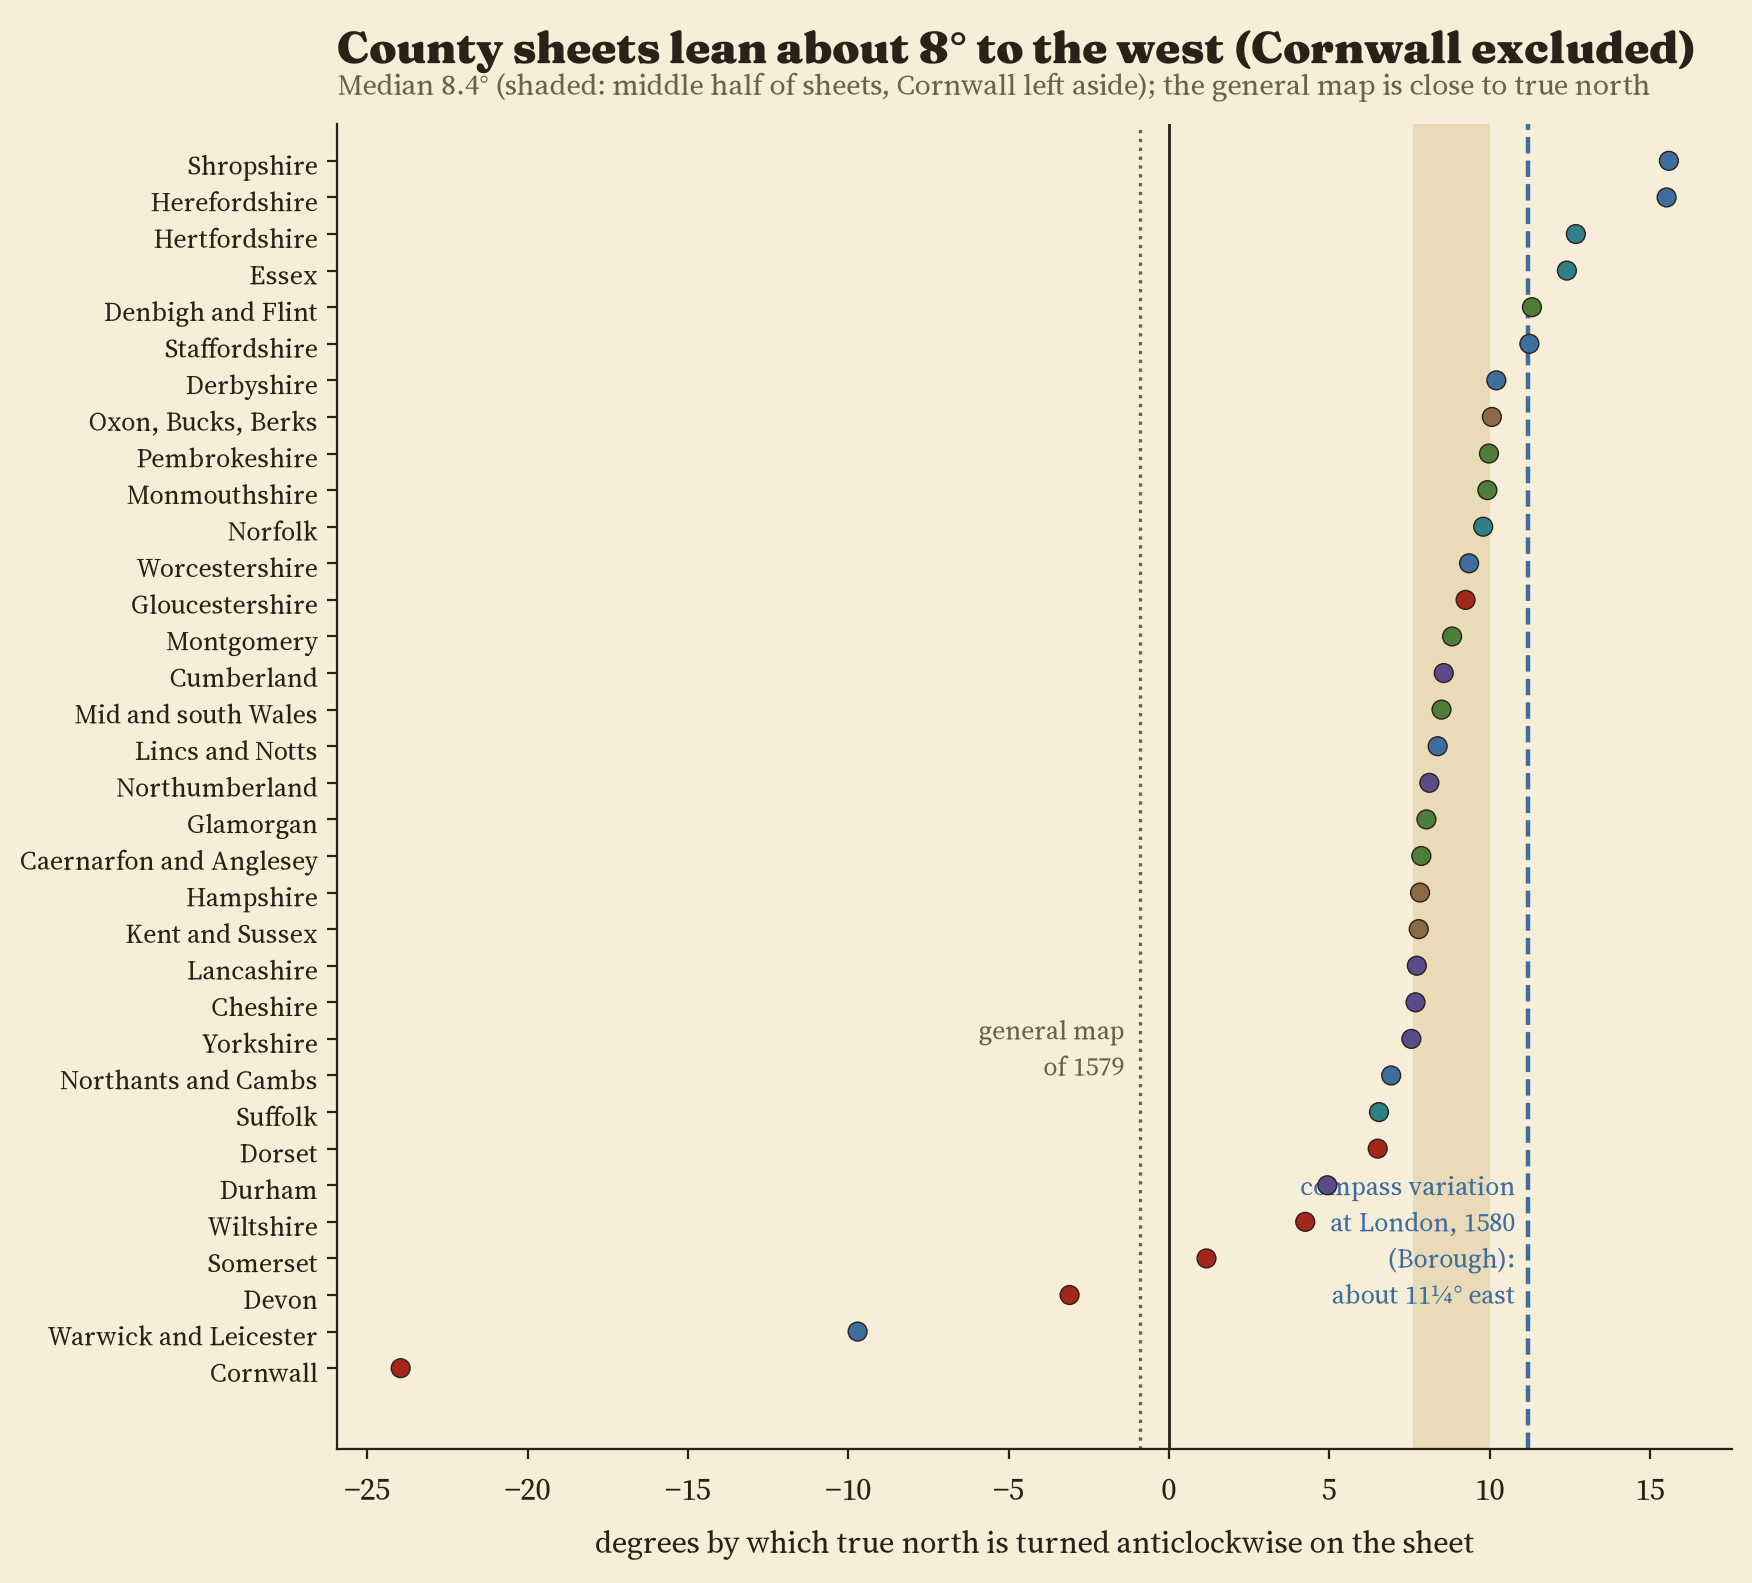
\includegraphics[width=.8\linewidth]{f_turns.png}\caption{Turn of true north on each county sheet, with Borough's 1580 value.}\end{figure}

\subsection{The general map and the Gough Map}
On the general map (46 towns) the median misplacement is 4.23 km (affine 4.08 km; 96\% within 10 km; largest Derby, 13.4 km), with a stretch of 1.02. The Gough Map of about 1360, measured with the same similarity fit, misplaces its median way station by 17.6 km \citep{gough}, 4.2 times as much. The comparison is rough: the samples of towns differ and the Gough Map includes Scotland's edge only through control points.
\begin{figure}[H]\centering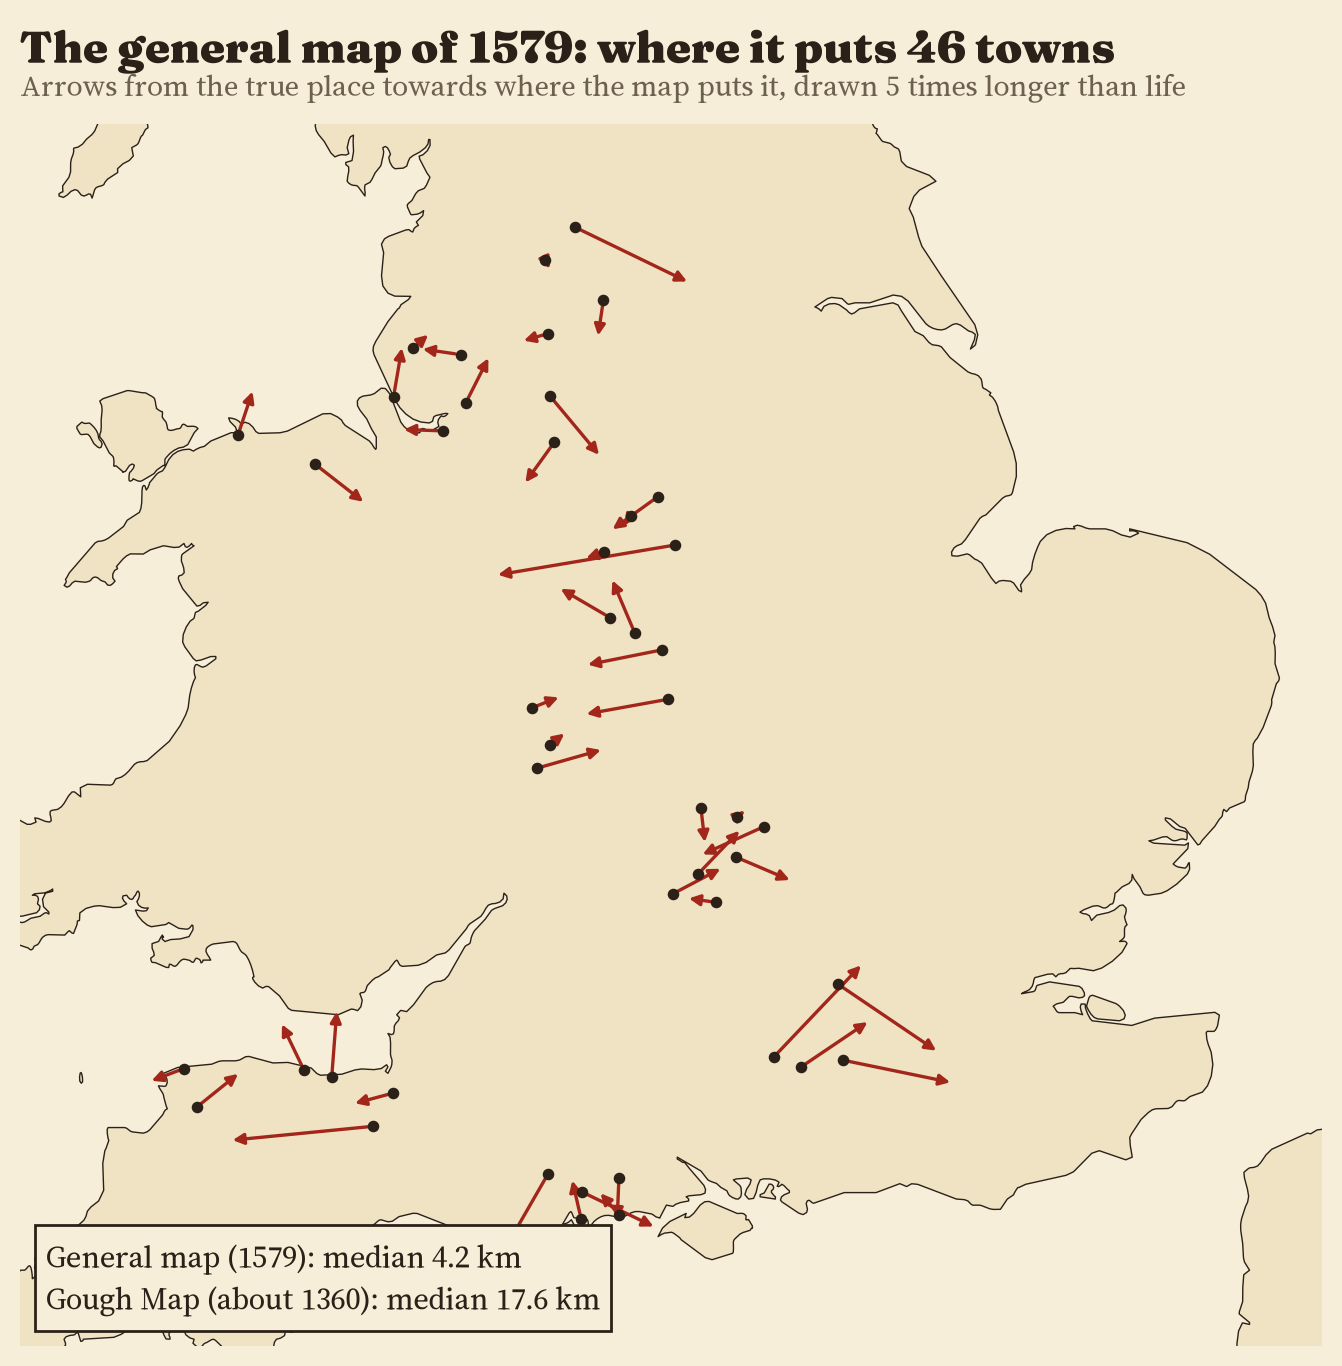
\includegraphics[width=.7\linewidth]{f_general.png}\caption{The general map of 1579: arrows from each true town towards its position on the map, five times exaggerated.}\end{figure}

\section{Limitations}
Readings are by eye and by one reader; names were matched to modern settlement points, not to historic church sites. Welsh sheets carry fewer places than most English ones. Small samples on some sheets (Pembrokeshire 7) make their medians uncertain. The scale bars on the sheets were not measured, so scales are given in scan pixels; the five duplicate sheets from other copies were not compared with the BnF impressions.

\section{Conclusion}
Saxton's county maps place towns typically within about one and a half kilometres of where an accurate map at the same scale and orientation would, with true shapes and consistent joins between neighbouring sheets. Their most striking systematic feature is the westward lean of north, of the size of the magnetic variation of the day, which the general map does not share. Two centuries after the Gough Map, the general map is about four times as accurate.

\section*{Data and code availability}
Data, code and the interactive page are at \url{https://github.com/Tristan-Hotham/saxton-atlas} and \url{https://maps.tristanhotham.com/saxton-atlas/}. Code MIT; text, figures and derived data CC BY 4.0. Wikidata is CC0; the scans are public domain.

\section*{AI statement}
I wrote the text, with drafting and editing assistance from Claude (Anthropic), which also helped prepare the analysis code. I reviewed and checked all text and results.

\begin{thebibliography}{9}
\bibitem[Bookstein(1989)]{bookstein} Bookstein, F. L. (1989) Principal warps: thin-plate splines and the decomposition of deformations. \emph{IEEE Transactions on Pattern Analysis and Machine Intelligence} 11(6), 567-585.
\bibitem[Borough(1581)]{borough} Borough, W. (1581) \emph{A Discours of the Variation of the Cumpas, or Magneticall Needle}. London.
\bibitem[Encyclopaedia Britannica(1911)]{eb1911} Encyclopaedia Britannica (1911) Magnetism, Terrestrial. 11th edn, vol. 17.
\bibitem[Evans and Lawrence(1979)]{evans} Evans, I. M. and Lawrence, H. (1979) \emph{Christopher Saxton, Elizabethan Map-maker}. Wakefield: Wakefield Historical Publications and Holland Press.
\bibitem[Hotham(2026)]{gough} Hotham, T. (2026) The Gough Map: Britain's oldest road map, measured. Zenodo. \url{https://doi.org/10.5281/zenodo.24043678}.
\bibitem[Natural Earth(n.d.)]{ne} Natural Earth. Free vector and raster map data. \url{https://www.naturalearthdata.com/}. Public domain.
\bibitem[Tobler(1994)]{tobler} Tobler, W. R. (1994) Bidimensional regression. \emph{Geographical Analysis} 26(3), 187-212.
\end{thebibliography}

\clearpage
\section*{Appendix: fits by sheet}
{\small\begin{longtable}{lrrrrrrrr}\toprule
Map & Year & $n$ & px/km & Sim. km & Aff. km & LOO km & Turn$^\circ$ & Stretch\\\midrule\endhead
General map & 1579 & 46 & 3.7 & 4.23 & 4.08 & 4.46 & -0.9 & 1.02 \\
Kent and Sussex & 1575 & 28 & 20.7 & 1.34 & 1.37 & 1.78 & +7.8 & 1.01 \\
Hampshire & 1575 & 21 & 26.6 & 1.62 & 1.62 & 2.45 & +7.8 & 1.08 \\
Dorset & 1575 & 19 & 34.2 & 0.97 & 0.94 & 1.22 & +6.5 & 1.05 \\
Wiltshire & 1576 & 28 & 29.2 & 1.15 & 0.78 & 1.06 & +4.2 & 1.10 \\
Somerset & 1575 & 22 & 29.7 & 1.29 & 1.31 & 1.05 & +1.2 & 1.02 \\
Devon & 1575 & 22 & 21.9 & 2.66 & 2.24 & 1.18 & -3.1 & 1.14 \\
Cornwall & 1576 & 20 & 21.7 & 1.60 & 1.60 & 1.27 & -24.0 & 1.02 \\
Essex & 1576 & 17 & 33.7 & 1.97 & 1.54 & 2.09 & +12.4 & 1.05 \\
Hertfordshire & 1577 & 24 & 46.1 & 1.27 & 1.17 & 1.51 & +12.7 & 1.09 \\
Oxon, Bucks, Berks & 1574 & 28 & 23.6 & 0.93 & 1.19 & 0.98 & +10.1 & 1.02 \\
Gloucestershire & 1577 & 24 & 24.2 & 1.34 & 1.26 & 1.10 & +9.2 & 1.07 \\
Suffolk & 1575 & 24 & 24.9 & 1.76 & 1.53 & 1.31 & +6.5 & 1.09 \\
Norfolk & 1574 & 24 & 23.7 & 2.01 & 1.93 & 1.33 & +9.8 & 1.03 \\
Northants and Cambs & 1576 & 36 & 22.3 & 2.00 & 1.95 & 1.59 & +6.9 & 1.04 \\
Warwick and Leicester & 1576 & 19 & 22.6 & 1.58 & 1.32 & 1.68 & -9.7 & 1.07 \\
Staffordshire & 1577 & 18 & 23.0 & 1.14 & 1.14 & 1.31 & +11.2 & 1.02 \\
Worcestershire & 1577 & 21 & 31.3 & 0.68 & 0.69 & 0.64 & +9.4 & 1.01 \\
Shropshire & 1577 & 19 & 29.3 & 1.07 & 0.97 & 1.37 & +15.6 & 1.03 \\
Herefordshire & 1577 & 26 & 35.0 & 0.81 & 0.82 & 0.97 & +15.5 & 1.08 \\
Lincs and Notts & 1576 & 28 & 19.5 & 1.65 & 1.65 & 1.58 & +8.4 & 1.00 \\
Derbyshire & 1577 & 20 & 28.2 & 0.69 & 0.76 & 1.04 & +10.2 & 1.02 \\
Cheshire & 1577 & 22 & 33.7 & 1.29 & 1.30 & 1.73 & +7.7 & 1.05 \\
Yorkshire & 1577 & 62 & 17.6 & 1.77 & 1.42 & 0.98 & +7.6 & 1.05 \\
Lancashire & 1577 & 24 & 19.5 & 1.40 & 1.27 & 1.96 & +7.7 & 1.02 \\
Durham & 1576 & 19 & 34.5 & 1.70 & 1.28 & 1.61 & +4.9 & 1.14 \\
Cumberland & 1576 & 16 & 20.4 & 1.63 & 1.24 & 1.26 & +8.6 & 1.05 \\
Northumberland & 1576 & 17 & 19.2 & 1.34 & 1.26 & 1.26 & +8.1 & 1.04 \\
Monmouthshire & 1577 & 25 & 41.1 & 1.16 & 0.79 & 0.89 & +9.9 & 1.14 \\
Glamorgan & 1578 & 15 & 33.9 & 1.12 & 0.93 & 1.51 & +8.0 & 1.10 \\
Mid and south Wales & 1578 & 48 & 22.1 & 2.17 & 1.85 & 1.47 & +8.5 & 1.07 \\
Pembrokeshire & 1578 & 7 & 32.5 & 1.04 & 1.13 & 1.55 & +10.0 & 1.05 \\
Montgomery & 1578 & 25 & 27.8 & 1.57 & 1.46 & 1.63 & +8.8 & 1.06 \\
Denbigh and Flint & 1577 & 25 & 34.0 & 1.38 & 0.85 & 0.89 & +11.3 & 1.16 \\
Caernarfon and Anglesey & 1578 & 18 & 24.4 & 1.83 & 1.39 & 1.55 & +7.9 & 1.08 \\
\bottomrule\end{longtable}}
\end{document}
